\documentclass[conference]{acmsiggraph}

\usepackage[utf8]{inputenc}  
\usepackage[T1]{fontenc}  

%%% Make the ``BibTeX'' word pretty...

\def\BibTeX{{\rm B\kern-.05em{\sc i\kern-.025em b}\kern-.08em
    T\kern-.1667em\lower.7ex\hbox{E}\kern-.125emX}}

\title{Procedurally Generating Content from Video Stream}

%%% TODO: Mettre les adresses de l'école
%%\author{Guillaume Ambrois\thanks{e-mail:guillaume.ambrois@gmail.com}, Sébastien %%Gaulier\thanks{e-mail:sebastien.gaulier@gmail.com}\\ESGI, Paris}
%%\pdfauthor{Guillaume Ambrois & Sébastien Gaulier}

\author{Anonym}
\pdfauthor{Anonym}

%%\keywords{procedural, computer vision}

\begin{document}

%%% This is the ``teaser'' command, which puts an figure, centered, below 
%%% the title and author information, and above the body of the content.

 \teaser{
   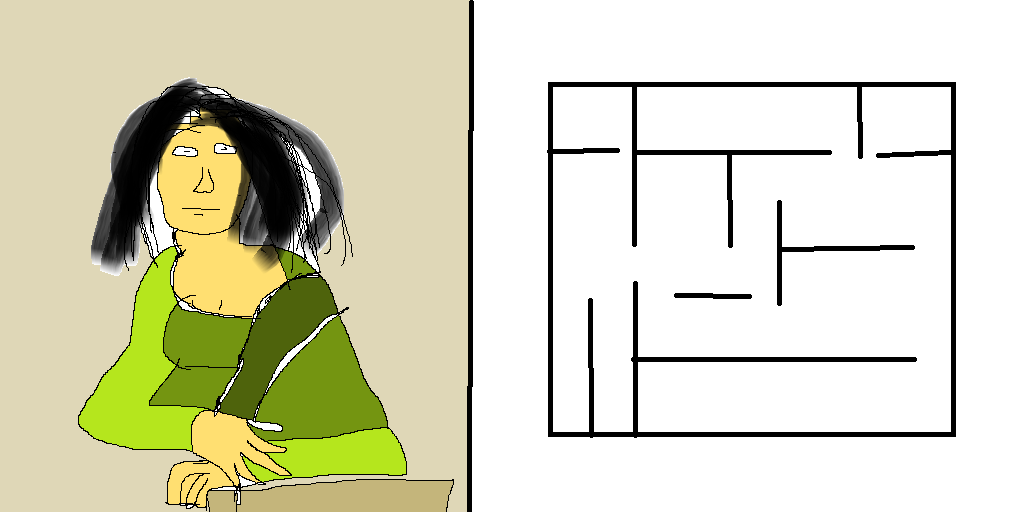
\includegraphics[height=1.5in]{images/sampleteaser}
   \caption{A procedurally generated map from an image}
 }

\maketitle

%% Required for all content. 

\copyrightspace

\section{Introduction}

Over the past years, procedurally generated content has become increasingly popular, especially in video games.
But the seed (the data used as input for the algorithm) for those procedural algorithms is almost always  just a number.

Meanwhile, computer vision algorithms keep getting faster, stronger and smarter.

And so we decided to try and mix the two together.

In this poster, we will explain the design we had in mind, and how we implemented it.

\section{Our approach}

We first had to decide what we wanted to look for in the video.
For this, we considered : 
\begin{itemize}
	\item Moving elements
	\item Changing colors
	\item Changing shapes
\end{itemize}

We decided to focus on detecting elements, and follow their movements, which is the thing the human eye is the best at doing.

Then, we had to decide what type of content we wanted to procedurally generate using those data.
The game we developed as a proof of concept was a multiplayer arcade game in which you wandered around a maze-like arena, collecting treasures and battling against other players and computer controlled characters.

The content we considered to procedurally generate were :
\begin{itemize}
	\item The layout of a level
	\item An IA behavior
	\item Player capacities
\end{itemize}

We went along with a procedurally generated level. Even if it's not really original, it's with this that we will have the most noticeable and interesting results.

\section{Technical implementation}

In our project, we used Unreal Engine 4 as game engine, and OpenCV 3.1 to process the video from which we want to extract data.

Firstly, for the sake of simplicity, we used short videos (2 to 3 minutes), with a static point of view to get rid of the complexity of keeping track of the camera's movement.

At the start of the video, we select a few elements we want to track, and we create a room with a random size for each element.

Then, we process each frame of the video in real time, trying to follow the motion of the elements we're tracking and changing the room size depending on the size of the associated element (some proportionally, some inversely proportional).

Finally, to add some personality, depending on the dominant color in the image, the theme of the level will change. For example, a dominantly red image will give a lava theme, while a dominantly green image will give a forest theme, with a grassy ground, bushes and trees.

\bibliographystyle{acmsiggraph}
\nocite{*}
\bibliography{abstract}
\end{document}
